%!LW recipe=pdflatex -> bibtex -> pdflatex -> pdflatex
\documentclass[conference, letterpaper]{IEEEtran}
\usepackage{cite}
\usepackage{amsmath,amssymb,amsfonts}
\usepackage{algorithmic}
\usepackage{graphicx}
\usepackage{textcomp}
\usepackage{xcolor}
\usepackage{blindtext}
\usepackage{booktabs}
\usepackage{bm}

\def\BibTeX{{\rm B\kern-.05em{\sc i\kern-.025em b}\kern-.08em
    T\kern-.1667em\lower.7ex\hbox{E}\kern-.125emX}}
\begin{document}

\title{Experimental Determination of Mechanical Properties of Metal Specimens}

\author{\IEEEauthorblockN{Jamie Kang}}

\maketitle

\section{Introduction}
    Materials testing is pivotal for understanding the mechanical behavior of materials, and stress-strain curves are fundamental tools in this regard. The distinction between engineering and true stress-strain curves, based on initial vs. instantaneous cross-sectional areas, becomes particularly significant when materials deform, especially in ductile materials prone to necking. This study aims to use experimental methods to find the mechanical properties of given specimens.

\section{Materials and Methods}
    Following the lab manual~\cite{2OLM2023}, the specimen's dimensions were measured with a vernier caliper, and the gauge length was marked. Subsequently, the specimen was loaded into the PASCO Materials Testing System, undergoing a 150N preload. It was then loaded to 1000N, with diameter and displacement recorded, and loaded to failure. Data from another team's specimen were acquired for comparison. Engineering stress-strain curves, critical stress values, Young's moduli, and Poisson's ratios were calculated from data files exported from the PASCO Materials Testing System using MATLAB for both specimens. Henceforth, the author's tested specimen is denoted as specimen 1, and the other group's tested specimen as specimen 2.

\section{Results}

    Engineering stress-strain curves for both specimens, along with yield stresses determined using the 0.02 offset method, are presented in Fig.~\ref{fgr_1}.

    \begin{figure}[htbp]
        \centerline{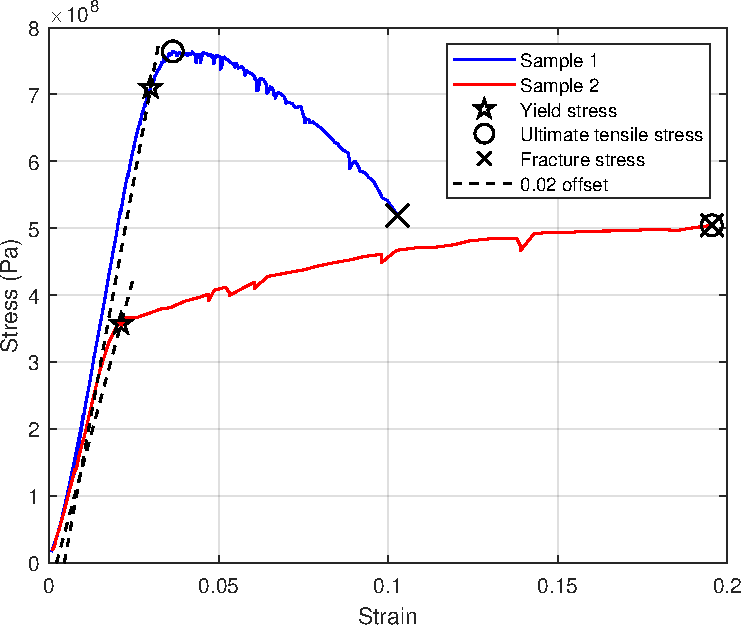
\includegraphics[width = \linewidth]{lab2curve.pdf}}
        \caption{Stress-strain curve, 0.02 parallel offset line, and important stress values for both specimens.}\label{fgr_1}
    \end{figure}

    \vspace*{-\baselineskip}
    \begin{table}[htbp]
        \caption{Percent Changes in Gauge Length, Young's Modulus, Yield Stress, Ultimate Tensile Stress, Fracture Stress, Possion's Ratio, and Density for Both Specimens}
        \begin{minipage}{\linewidth}
            \centering
            \begin{tabular}{lcc}
                \toprule{}
                & \textbf{Specimen 1} & \textbf{Specimen 2} \\
                \midrule{}
                \hspace*{-1ex}\textbf{\% Change Gauge Length (G)} & 11\% & 11\% \\
                \textbf{Young's Modulus (E)} & 27.883 GPa & 18.785 GPa \\
                \textbf{Yield Stress (\(\bm{\sigma_y}\))} & 710.073 MPa & 357.379 MPa \\
                \textbf{Ultimate Tensile Stress (\(\bm{\sigma_u}\))} & 764.309 MPa & 504.502 MPa\\
                \textbf{Fracture Stress (\(\bm{\sigma_f}\))} & 519.126 MPa & 504.502 MPa \\
                \textbf{Poisson's Ratio (\(\bm{\upsilon}\))} & 0.919 & 0\footnote{According to data received from other group, no difference in diameter could be measured from the vernier caliper used.} \\
                \textbf{Density} & 8.443 g/cm\textsuperscript{3} & 2.997 g/cm\textsuperscript{3} \\
                \bottomrule{}
            \end{tabular}\label{tbl_1}
            \vspace*{-\baselineskip}
        \end{minipage}
    \end{table}
    Sample calculations can be found in Appendix\ \ref{apdx_1}.

\section{Discussion}
    In this experiment, we plotted engineering stress-strain curves, which differ from true stress-strain curves in how they are calculated. 
    Engineering stress relies on the initial area, while true stress considers the instantaneous cross-sectional area as the load is applied to the specimen. 
    This distinction leads to higher true stress values compared to engineering stress, and it becomes particularly significant for ductile materials as they undergo necking, causing the cross-sectional area to decrease after reaching ultimate stress.

    However, it was impractical to plot true stress-strain curves in this experiment due to the continuous measurement of the sample's diameter required as it undergoes strain. 
    The PASCO Materials Testing System used in the experiment lacks the capability to measure the sample's diameter in real-time as the load is applied, and manual measurement would be both time-consuming and impractical. 
    Moreover, in the elastic region, the difference between engineering and true stress is negligible, and this region is where crucial material properties such as Young's modulus and yield stress are determined.

    For identifying the two materials tested, we used data from Table~\ref{tbl_1} and compared Young's modulus, Poisson's ratio, and density with common engineering metals as specified in the textbook~\cite{Hibbeler2022}. 
    Unfortunately, the calculated Young's modulus and Poisson's ratio did not correspond to known engineering metals. 
    This discrepancy may be attributed to grooves marked on the specimen during gauge length marking, potentially weakening the material and leading to inaccurate results. 
    As a result, we inferred that specimen 1 is ductile cast iron, characterized by its dark silver or grey appearance and a density of 7.30g/cm\textsuperscript{3}. 
    Specimen 2 is most likely aluminum alloy 7075, known for its high strength but reduced ductility, with a density of 2.80g/cm\textsuperscript{3}. 
    Notably, specimen 1 exhibited greater ductility, as evident from its stress-strain curve, while specimen 2 failed almost immediately after reaching ultimate stress, indicating a more brittle behavior. 
    This suggests that specimen 1 is better suited for applications requiring ductility, while specimen 2 is more appropriate for situations where strength takes precedence over ductility.

\bibliographystyle{ieeetran}
\bibliography{lab2}

\appendices{}

\section{Sample Calculations}\label{apdx_1}
    All sample calculations are for Specimen 1.
    \subsection{Percent Change in Gauge Length}
        The gauge length is 0.02m. When \(\Delta \) displacement is \(1.452(10^{-4})\)m, strain is:
        \[
            \varepsilon \;
            =\; \frac{\Delta L}{L_0} \;
            =\; \frac{(1.452(10^{-4})\text{m})}{(0.02\text{m})} \;
            =\; 7.26(10^{-3})
        \]
    \subsection{Strain}
        The gauge length is 0.02m. When \(\Delta \) displacement is \(1.452(10^{-4})\)m, strain is:
        \[
            \varepsilon \;
            =\; \frac{\Delta L}{L_0} \;
            =\; \frac{(1.452(10^{-4})\text{m})}{(0.02\text{m})} \;
            =\; 7.26(10^{-3})
        \]
    \subsection{Engineering Stress}
        The initial diameter is 0.00336m. When force is 1149N, engineering stress is:
        \[
            \sigma \;
            =\; \frac{F}{A_0} \;
            =\; \frac{(1149\text{N})}{\frac{\pi}{4} {(0.00336\text{m})}^2} \;
            =\; 129.584\ \text{MPa}
        \]
    \subsection{Young's Modulus}
        Linear regression was calculated using formula from Statstical Methods by Snedecor and Cochran\cite{SNEDECOR1989} on linear portion of data collected:
        \[
            \hat{Y} = b_0 + b_{1}X.
        \]
        Coefficients of the intercept and slope, calculated using the / operator on MATLAB:\@
        \begin{align*}
            b_0
            &= -70139053.3117333 \\
            b_1
            &= 27883474684.1003
        \end{align*}
        Slope \(b_1\) was used as Young's Modulus:
        \begin{align*}
            E
            &= 27883474684.1003\ \text{Pa} \\
            &= 27.883\ \text{GPa}
        \end{align*}
    \subsection{0.2\% Offset Yield Stress}
        Material does not have a well-definied elastic limit; thus, the 0.2\% parallel offset method\cite{Hibbeler2022} was used to find the yield point.
        \[
            \hat{Y} = b_0 + b_{1}(X-0.002)
        \]
        The above function was plotted, and the resulting intersection point (Fig.\ \ref{fig2}) with the stress-strain curve was used to find the yield stress:
        \begin{align*}
            \sigma_y 
            &= 710073000\ \text{Pa} \\
            &= 710.073\ \text{MPa}
        \end{align*}
        \vspace*{-\baselineskip}
        \begin{figure}[htbp]
            \centerline{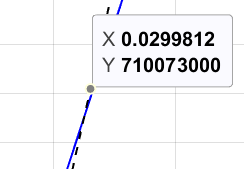
\includegraphics[width = 2in]{figures/intersection1.png}}
            \caption{Intersection point between 0.2\% offset line and stress-strain curve.}\label{fig2}
            \end{figure}
    \subsection{Poisson's Ratio}
        When 1149N of force was applied to the Specimen,
        \begin{align*}
            \varepsilon_{lat} 
            &= \frac{-0.00002\text{m}}{0.00336\text{m}} = -0.005952380952381 \\
            \varepsilon_{long}
            &= \frac{0.00012954\text{m}}{0.02\text{m}} = 0.006477000000000
        \end{align*}
        Thus, possion's ratio is
        \[
            \nu = - \frac{\varepsilon_{lat}}{\varepsilon_{long}}
            = 0.919
        \]
\end{document}